\documentclass[tikz,border=5]{standalone}
\usetikzlibrary{decorations.pathmorphing}
\usepackage[detect-all]{siunitx}

\tikzset{
   ragged border/.style={ decoration={random steps, segment length=1mm, amplitude=0.5mm},
           decorate,
   }
}

\begin{document}
  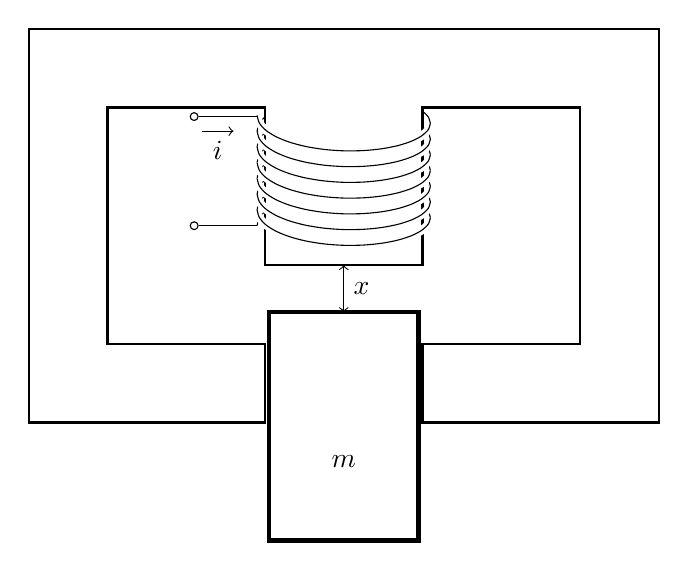
\begin{tikzpicture}
  \draw[thick] (0,0) -- (0,5) -- (8,5) -- (8,0) -- (5,0) -- (5,1) -- (7,1) -- (7,4) -- (5,4) -- (5,2) -- (3,2) -- (3,4) -- (1,4) -- (1,1) -- (3,1) -- (3,0) -- cycle;

  
   % Define a formula for the coil.
    % This is what the numbers mean:
    % 0.3 ... how far the rings are apart
    % 0.4 ... how much from the side the rings are seen (try 0 and the same as the radius)
    % 1.5 ... radius of the rings
    \def\coil#1{
        {0.1 * (2*#1 + \t) + 0.4*sin(\t * pi r))},
        {1.1 * cos(\t * pi r)}
        }

    \begin{scope} [rotate=90, yshift=-4cm, xshift=2.5cm]
    % Draw the part of the coil behind the rectangle
    \foreach \n in {0,1,...,6} {
        \draw[domain={0:1},smooth,variable=\t,samples=15]
            plot (\coil{\n}); 
        }

    % Draw the rectangle
    \filldraw[fill=white, white] (-0.2,-0.98) rectangle (1.95,0.98);

    % Draw the part of the coil in front of the rectangle
    \foreach \n in {0,1,...,6} {
        \draw[domain={1:2},smooth,variable=\t,samples=15,
              preaction={draw,white,line width=3pt}     % remove if undesired
             ]
            plot (\coil{\n});
        }
 \end{scope}
 
 \node[circle, draw, inner sep=1pt] (terminal1) at (2.1, 3.885) {};
 \node[circle, draw, inner sep=1pt] (terminal2) at (2.1, 2.499) {};

 \draw[] (terminal1) -- (2.9, 3.885);
 \draw[->] (2.2, 3.7) -- node[below] {$i$} (2.6, 3.7);

 \draw (terminal2) -- (2.9, 2.499);

 \draw[ultra thick] (3.05, -1.5) -- (3.05, 1.4) -- (4.95, 1.4) -- (4.95, -1.5) -- cycle;

 \draw[<->] (4, 1.4) -- node [right] {$x$} (4, 2);
 
 \node at (4, -0.5) {$m$};

\end{tikzpicture}%
\end{document}